\documentclass[12pt,titlepage]{article}
\usepackage[margin=1.25in]{geometry}
\usepackage{graphicx,amsmath,blindtext,minted}

%% Variables definition
\newcommand{\vSubject}{Basic Programming Practicum}
\newcommand{\vSubtitle}{Function 2 Recursion}
\newcommand{\vName}{Dicha Zelianivan Arkana}
\newcommand{\vNIM}{2241720002}
\newcommand{\vClass}{1i}
\newcommand{\vDepartment}{Information Technology}
\newcommand{\vStudyProgram}{D4 Informatics Engineering}

%% [START] Tikz related stuff
\usepackage{tikz}
\usetikzlibrary{svg.path,calc,shapes.geometric,shapes.misc}
\tikzstyle{terminator} = [rectangle, draw, text centered, rounded corners = 1em, minimum height=2em]
\tikzstyle{preparation} = [chamfered rectangle, chamfered rectangle sep=0.75em, draw, text centered, minimum height = 2em]
\tikzstyle{process} = [rectangle, draw, text centered, minimum height=2em]
\tikzstyle{decision} = [diamond, aspect=2, draw, text centered, minimum height=2em]
\tikzstyle{data}=[trapezium, draw, text centered, trapezium left angle=60, trapezium right angle=120, minimum height=2em]
\tikzstyle{connector} = [line width=0.25mm,->]
%% [END] Tikz related stuff

%% [START] Fancy header related stuff
\usepackage{fancyhdr}
\pagestyle{fancy}
\setlength{\headheight}{15pt} % compensate fancyhdr style
\fancyhead{}
\fancyfoot{}
\fancyfoot[L]{\thepage}
\fancyfoot[R]{\textit{\vSubject - \vSubtitle}}
\renewcommand{\footrulewidth}{0.4pt}% default is 0pt, overline for footer
%% [END] Fancy header related stuff

%% [START] Custom tabular command related stuff
\usepackage{tabularx}
\newcommand{\details}[2]{
    #1 & #2  \\
}
%% [END] Custom tabular command related stuff

%% [START] Figure related stuff
\newcommand{\image}[3][1]{
    \begin{figure}[h]
        \centering
        \includegraphics[#1]{#2}
        \caption{#3}
        \label{#3}
    \end{figure}
}
%% [END] Figure related stuff

\begin{document}
\begin{titlepage}
    \centering
    \vfill
    {\bfseries\LARGE
        \vSubject\\
        \vskip0.25cm
        \vSubtitle
    }
    \vfill
    
\includegraphics[width=6cm]{images/polinema-logo.png}
    \vfill
    {
        \textbf{Name}\\
        \vName\\
        \vskip0.5cm
        \textbf{NIM}\\
        \vNIM\\
        \vskip0.5cm
        \textbf{Class}\\
        \vClass\\
        \vskip0.5cm
        \textbf{Department}\\
        \vDepartment\\
        \vskip0.5cm
        \textbf{Study Program}\\
        \vStudyProgram
    }
\end{titlepage}

\section{Laboratory}
\subsection{Experiment 1}
In this experiment, a program will be created to calculate the factorial value of a number using a recursive function.
In addition, a function for calculating factorial values will be made using an iterative algorithm as a comparison.
\begin{enumerate}
    \item Create a new project
    \item Create a new class, name it \textbf{Experiment}
    \item {
        Create a static function with the name \texttt{factorialRecursive()}, 
        with return data type that is \texttt{int} and has 1 parameter with \texttt{int} data type in the form of a number calculated for its factorial value.

        \begin{minted}[autogobble]{java}
            static int factorialRecursive(int n) {
                if (n == 0) {
                    return 1;
                } else {
                    return n * factorialRecursive(n - 1);
                }
            }
        \end{minted}
    }
    \item {
        Create another static function with the name \texttt{factorialIterative()}, with return data type
        that is \texttt{int} and has 1 parameter with \texttt{int} data type in the form of a number calculated for its factorial value.

        \begin{minted}[autogobble]{java}
            static int factorialIterative(int n) {
                int factor = 1;
                for (int i = n; i >= 1; i++) {
                    factor = factor * i;
                }
                return factor;
            }
        \end{minted}
    }
    \item {
        Create a \texttt{main} function and make a call to the two previously created functions, 
        and display the results obtained.
    }
    \pagebreak
    \item {
        Compile and run the program

        \begin{figure}[h]
            \centering
            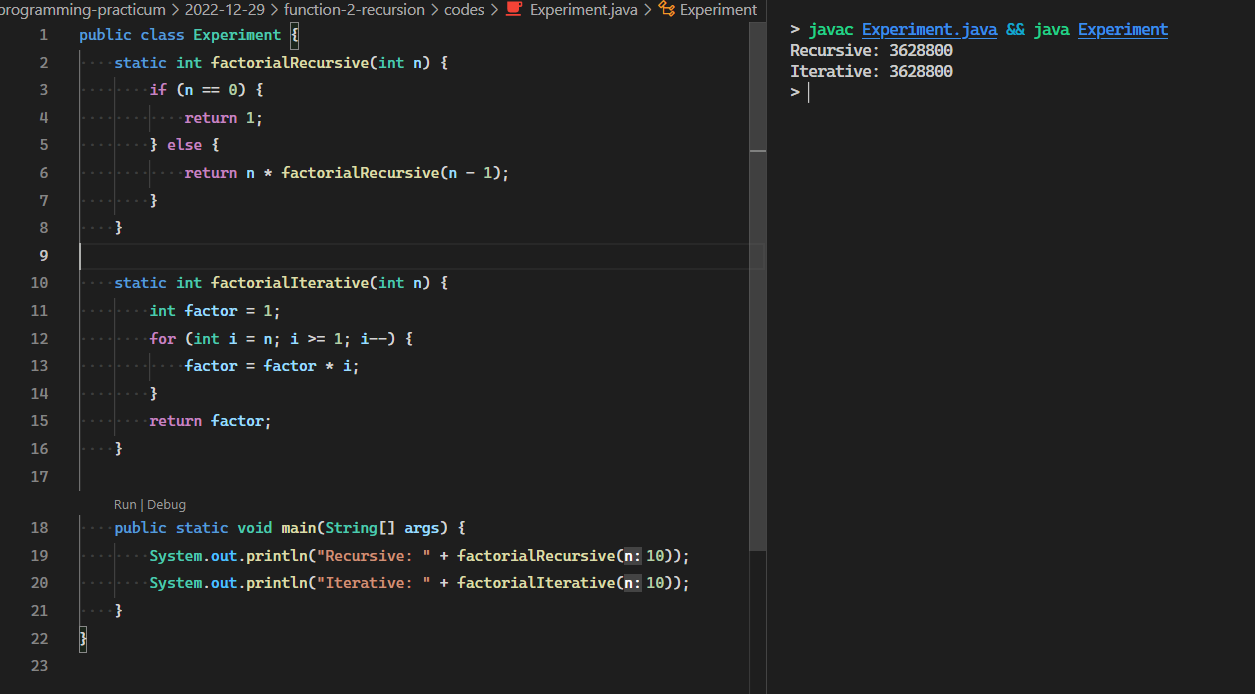
\includegraphics[width=\textwidth]{./images/experiment-one.png}
            \caption{Experiment 1 code and output}
        \end{figure}
    }
    \item {
        If traced, when calling the \texttt{factorialRecursive(5)} function, the process that occurs can be illustrated as follows:

        \begin{figure}[h]
            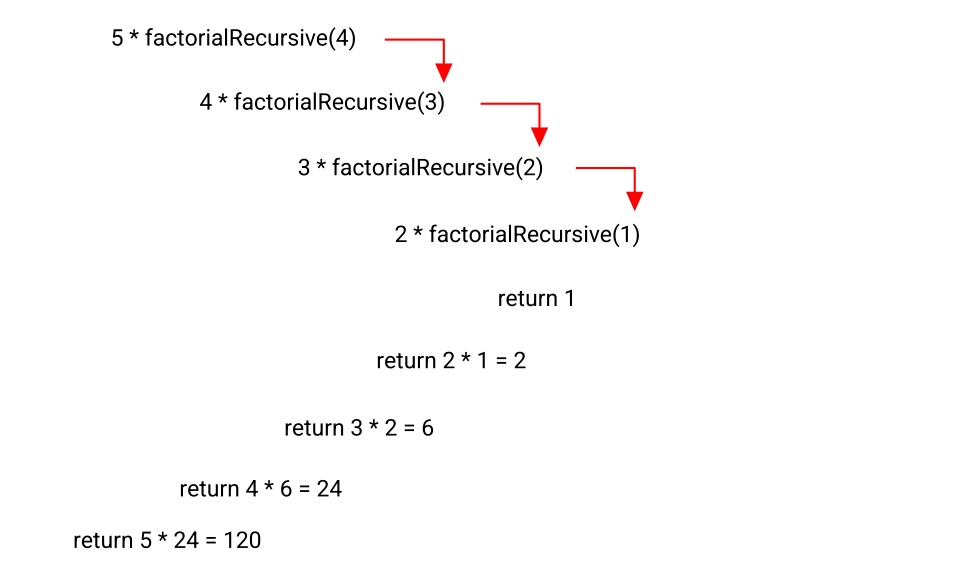
\includegraphics[width=.55\textwidth]{./images/trace.png}
            \caption{Traced recursive function}
        \end{figure}
    }
\end{enumerate}

\pagebreak

\subsection{Experiment 2}
In this experiment, a program will be created to calculate the power of a number using a recursive function.
\begin{enumerate}
    \item Create a new class, name it \texttt{Experiment2}
    \item {
        Create a static function with the name \texttt{calculatePower()}, with return data type
        that is \texttt{int} and has 2 parameter with \texttt{int} data type in the form of numbers to be
        calculated and the exponents.

        \begin{minted}[autogobble]{java}
            static int calculatePower(int x, int y) {
                if (y == 0) {
                    return 1;
                } else {
                    return x * calculatePower(x, y - 1);
                }
            }
        \end{minted}
    }
    \item Create a \texttt{main} function and declare a \texttt{Scanner} with the name \texttt{sc}
    \item Create two variables of type int with name \texttt{number} and \texttt{exponent}
    \item {
        Add the following code to accept input from the keyboard
        \begin{minted}[autogobble]{java}
            System.out.print("Enter a number: ");
            number = sc.nextInt();
            System.out.print("Enter the exponent: ");
            exponent = sc.nextInt();
        \end{minted}
    }
    \item {
        Call the \texttt{calculatePower} function that was created previously by sending two parameter values.
        \begin{minted}[autogobble]{java}
            System.out.println(calculatePower(number, exponent));
        \end{minted}
    }
    \pagebreak
    \item {
        Compile and run the program

        \begin{figure}[h]
            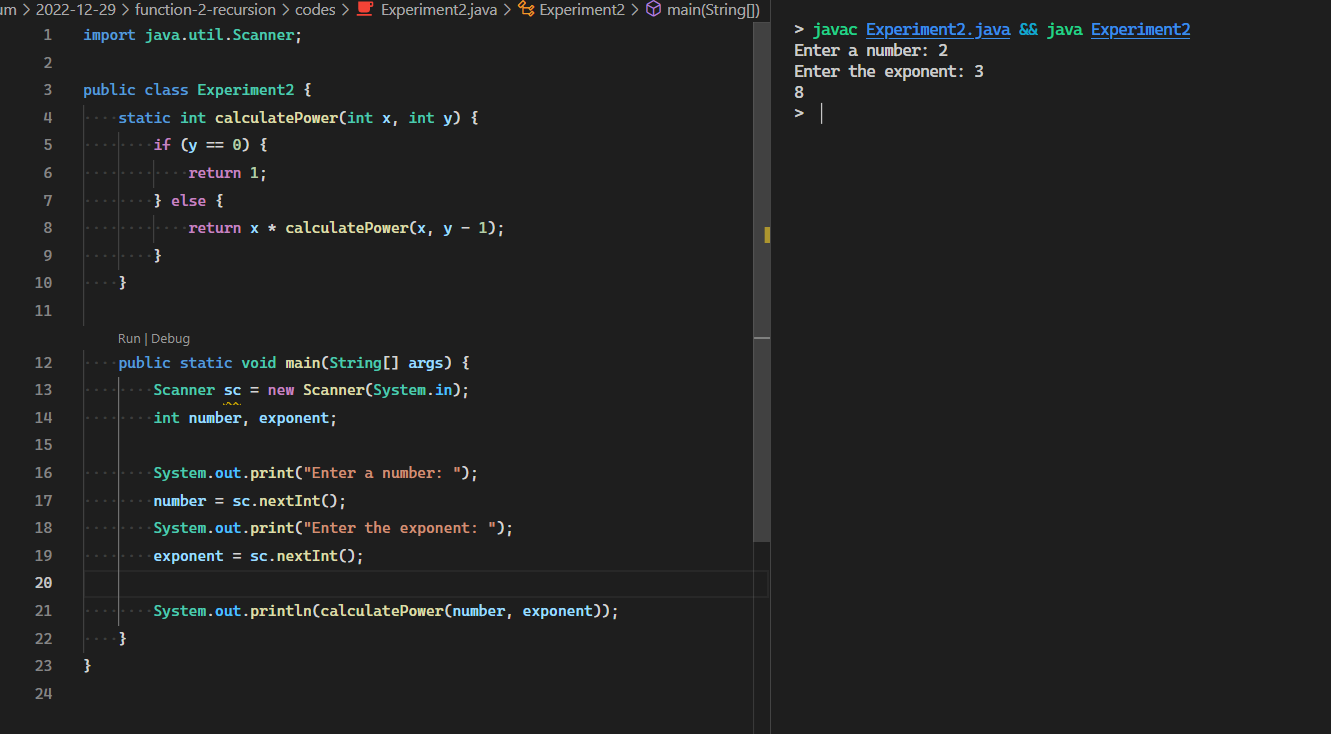
\includegraphics[width=\textwidth]{./images/experiment-two.png}
            \caption{Experiment 2 code and output}
        \end{figure}
    }
\end{enumerate}

\subsection{Experiment 3}
In this experiment, a program will be created to calculate the amount of customer money deposited in the bank after earning interest 
for several years using the recursive function
\begin{enumerate}
    \item Create a new class, name it \texttt{Experiment3}
    \item {
        Create a static function with the name \texttt{calculateInterest()}, with return data type
        that is double and has 2 parameter with \texttt{int} data type \texttt{int} in the form of customer
        balance and time spent saving. In this case, it is assumed that the interest set by the bank is 11\% annually. 
        Because the interest calculation is $interest * balance$, so to calculate the amount
        of money after adding interest is $balance + interest * balance$. In this case, the
        interest rate is $0.11 * balance$, and the balance is considered $1 * balance$, so $1 *
        balance + 0.11 * balance$ can be summarized into $1.11 * balance$ for calculating
        the balance after adding interest (in a year).

        \begin{minted}[autogobble]{java}
            static double calculateInterest(double balance, int year) {
                if (year == 0) {
                    return balance;
                } else {
                    return 1.11 * calculateInterest(balance, year - 1);
                }
            }
        \end{minted}
    }
    \item Create a main function and declare a \texttt{Scanner} with the name \texttt{sc}
    \item Create a variable of type double named \texttt{openingBalance} and a variable of type \texttt{int} named \texttt{year}
    \item {
        Add the following code to accept input from the keyboard

        \begin{minted}[autogobble]{java}
            System.out.print("Enter the opening balance: ");
            openingBalance = sc.nextDouble();
            System.out.print("Enter the duration of saving (years): ");
            year = sc.nextInt();
        \end{minted}
    }
    \item {
        Call the \texttt{calculateInterest} function that was created previously by sending two parameter values

        \begin{minted}[autogobble]{java}
            System.out.print("Amount of money after " + year + " years: ");
            System.out.println((int) calculateInterest(openingBalance, year));
        \end{minted}
    }
    \item {
        Compile and run the program

        \begin{figure}[h]
            \centering
            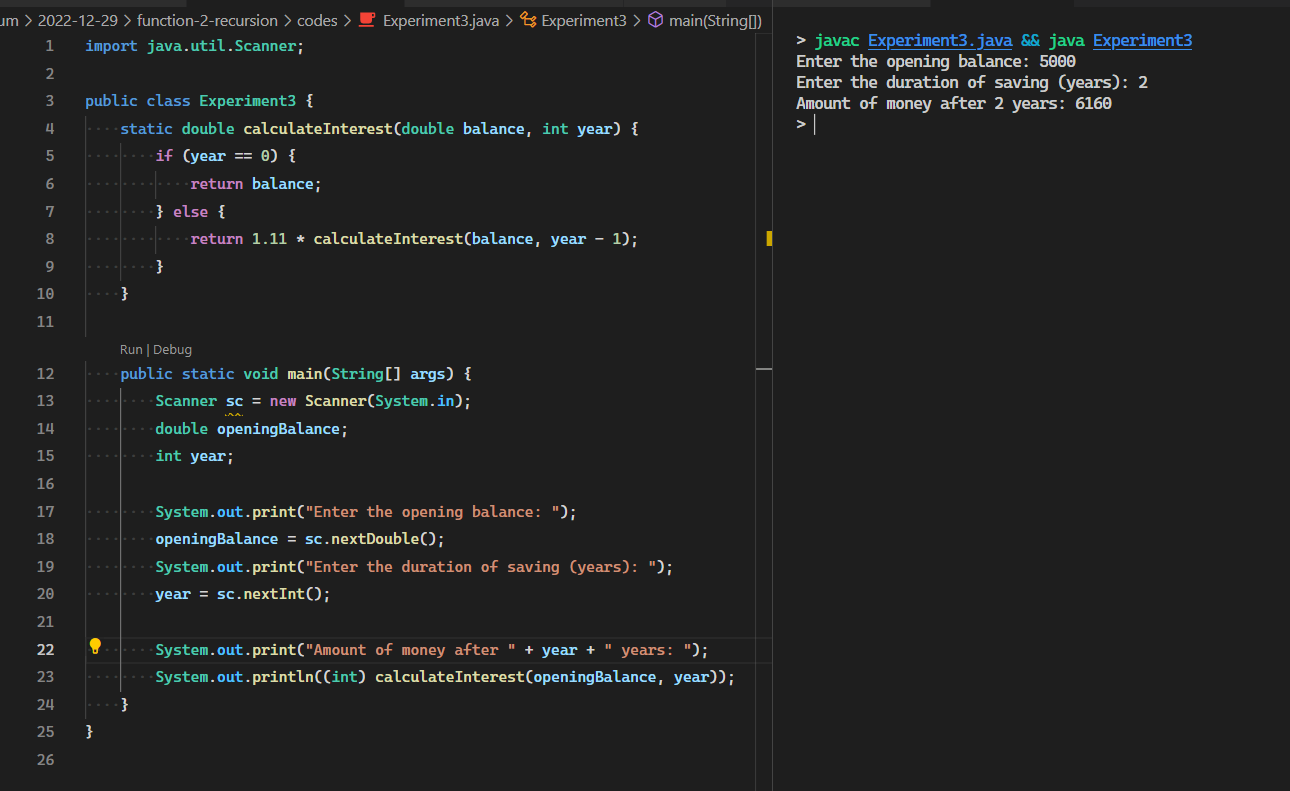
\includegraphics[width=.8\textwidth]{./images/experiment-three.png}
            \caption{Experiment 3 code and output}
        \end{figure}
    }
\end{enumerate}

\pagebreak

\subsection*{Questions!}
\begin{enumerate}
    \item {
        What is a recursive function?

        It's a type of function that calls itself. Though, it usually has base case that makes it stop, similar to an iterative loop.
    }
    \item {
        What are the examples of recursive functions?

        A function to calculate a factorial.
    }
    \item {
        In \textbf{Experiment 1}, do the \texttt{factorialRecursive()} function \\and \texttt{factorialIterative()}
        function give the same result? Explain the difference in the flow of the program in the use of recursive functions and iterative functions!

        The results are the same because they both are trying to do the same thing. The difference is how they achieve it. The former uses a recursive method while the latter uses the iterative method.
        The recursive method calls itself but changing the argument on each recursion.
    }
    \item {
        In \textbf{Experiment 2}, there is a recursive function call \texttt{calculatePower(number, exponent)} in the main function,
        then the \texttt{calculatePower()} function calls are repeated. Explain how long the function calling process will be executed!

        The function will be executed as long as the exponent doesn't reach 0. If it reaches zero then it will stop. For example, if the exponent is 5 then it will stop after the 5th recursion.
    }
    \item {
        In \textbf{Experiment 3}, state which program code block is the "base case" and "recursion call"!

        The condition that states \texttt{if (year == 0)} is the base case because it returns a plain value while the else block is the recursion value
        because it returns the result of the invocation of itself.
    }
\end{enumerate}

\pagebreak

\section{Assignment}
\begin{enumerate}
    \item {
        Create a program to display the numbers n through 0 using recursive and iterative functions. (\textbf{RecursiveDescendingSeries})

        \begin{figure}[h]
            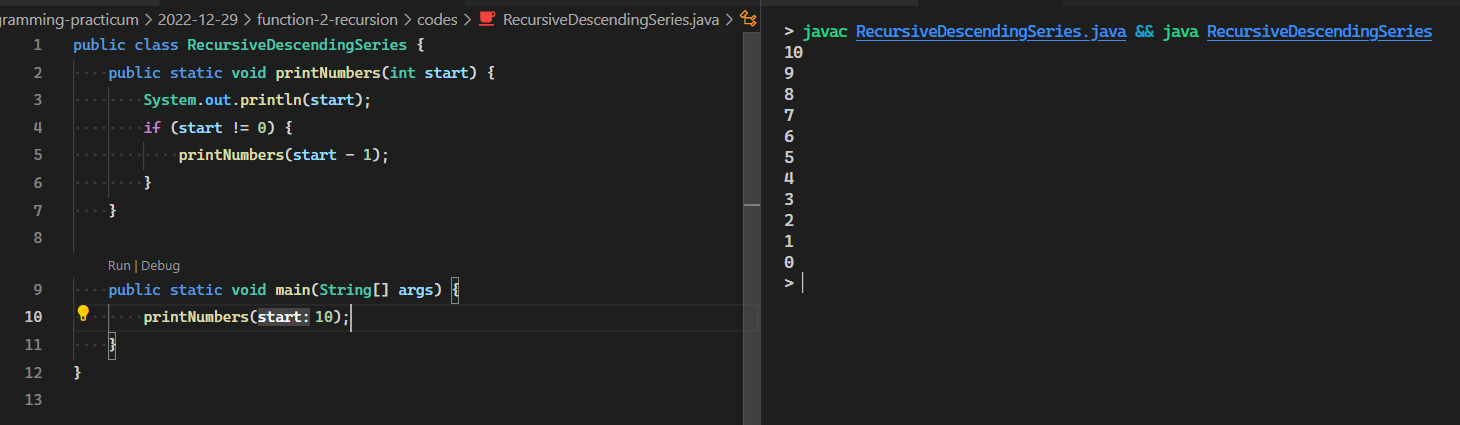
\includegraphics[width=\textwidth]{./images/assignment-one.png}
            \caption{Assignment 1 code and output}
        \end{figure}
    }
    \item {
        Create a program that includes a recursive function for calculating factorial numbers. For example, \texttt{f = 8}, it will produce \texttt{1 + 2 + 3 + 4 + 5 + 6 + 7 + 8 = 36}
        (\textbf{RecursiveAddition})

        \begin{figure}[h]
            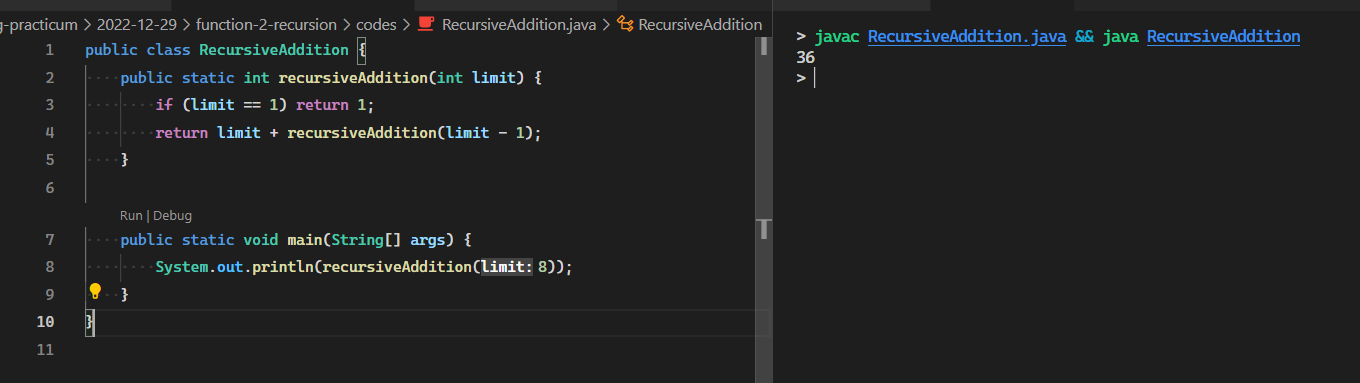
\includegraphics[width=\textwidth]{./images/assignment-two.png}
            \caption{Assignment 2 code and output}
        \end{figure}
    }
    \pagebreak
    \item {
        Create a program that includes a recursive function to check whether a number n is a prime number or not. n is said to be not a prime number if it is evenly divided by a number less than n
        (\textbf{RecursivePrimeCheck})

        \begin{figure}[h]
            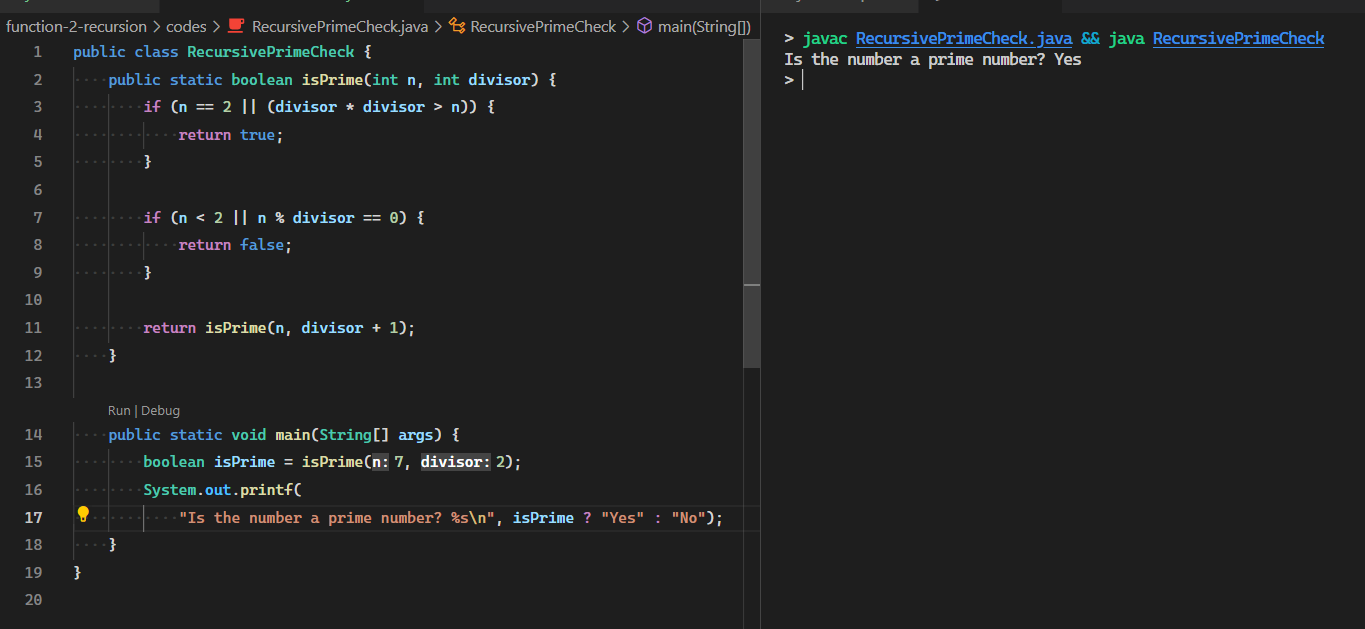
\includegraphics[width=\textwidth]{./images/assignment-three.png}
            \caption{Assignment 3 code and output}
        \end{figure}
    }
\end{enumerate}
 
\end{document}

